\section{Le Tore $T^2$}
\subsection{Première définition}
On définit le tore par $T^2=S^1\times S^1$, avec $S^1$ la sphère unité du plan (donc le cercle). Intuitivement, on fait tourner le $2$e cercle autour du $1$er, donnant une forme d'anneau :
\begin{figure}[h]
    \centering
    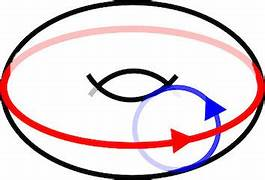
\includegraphics[width=0.2\textwidth]{images/Tore image.jpg}
    \caption{Le $1$er cercle en rouge, le $2$e en bleu}
\end{figure}
\bigskip\\
Il y a une manière assez directe de calculer le groupe fondamental de $\pi_1$ du tore, mais elle n'implique pas Van Kampen. On la donnera plus loin, car elle reste intéressante.
\begin{proposition}
    $T^2\cong I^2/\mathcal{R}$ avec $\mathcal{R}$ la relation d'équivalence engendrée par $(t,0)\sim(t,1)$ et $(0,t)\sim(1,t,),t\in[0,1]$.
\end{proposition}
\begin{proof}
    Soit $f:I^2\to T^2$ définie par $f(t,s)=(e^{2i\pi t},e^{2i\pi s})$ surjective et continue. Cette application passe au quotient car si $(t,s)\sim_R(t',s')$ on a $f(t,s)=f(t',s')$.\medskip\\
    On obtient alors $\overline{f}:[0,1]^2/\mathcal{R}\to T^2$ surjective, continue. Montrons qu'elle est injective : 
    Il suffit de montrer que si $f(t,s)=f(t',s')$, alors $(t,s)\sim_R(t',s')$. Or, on aurait $e^{2i\pi t}=e^{2i\pi t'}$ donc $t=t'$ ou $t,t'\in\{0,1\}$, et de même pour $s$ et $s'$. On a donc soit $(t,s)=(t',s')$, soit $t=t'$ et $s,s'\in\{0,1\}$ ou l'inverse. Dans tous les cas, $(t,s)\sim_R(t',s')$.\medskip\\
    $\overline{f}$ est bijective et continue, définie sur un compact donc bicontinue, donc c'est un homéomorphisme.
\end{proof}
On se situe maintenant dans le cadre pour lequel on a développé nos outils, et il ne reste plus qu'à procéder au calcul du groupe fondamental.
\subsection{Calcul par Van Kampen}
L'utilisation de Van Kampen pour le tore n'est pas la plus directe, comme on l'a déjà soulevé. Cependant, cela fait office d'un bon exercice, et d'une introduction à la méthode que l'on utilisera pour $\mathbb{R}$P$^2$ et la bouteille de Klein.
\begin{proposition}
    $\pi_1(I^2/\mathcal{R})\cong\mathbb{Z}^2$, induisant un isomorphisme entre $\pi_1(T^2)$ et $\mathbb{Z}^2$.
\end{proposition}
\begin{proof}
    En couvrant $I^2/\mathcal{R}$ par $\tilde{U}_0$ et $\tilde{V}_0$, le théorème de Van Kampen donne $\pi_1(I^2/\mathcal{R}) \cong \pi_1(\tilde{U}_0) * \pi_1(\tilde{V}_0) / N$ où $N$ est le sous-groupe normal engendré par les éléments $i_{\tilde{V}_0}(c) \cdot i_{\tilde{U}_0}(c)^{-1}$ pour $c$ parcourant $\pi_1(\tilde{U}_0 \cap \tilde{V}_0)$. Or $\tilde{U}_0$ est simplement connexe (Corollaire 2.1), donc $\pi_1(\tilde{U}_0)$ est isomorphe au groupe trivial, et on obtient $\pi_1(I^2/\mathcal{R}) \cong \pi_1(\tilde{V}_0)/N$.\medskip\\
    Les isomorphismes $\pi_1(\tilde{V}_0) \cong \pi_1(q(\partial I^2)) \cong \pi_1(S^1 \vee S^1) \cong \mathbb{Z} * \mathbb{Z}$ (Lemme 2.1, Proposition 2.4, Corollaire 2.2) induisent un isomorphisme $\phi : \pi_1(\tilde{V}_0) \rightarrow\mathbb{Z} * \mathbb{Z}$. L'isomorphisme $\phi$ induit alors $\pi_1(T^2) \cong \pi_1(\tilde{V}_0)/N \cong \mathbb{Z}*\mathbb{Z}/\phi(N)$. On note $\alpha$ et $\beta$ respectivement les classes des lacets $t \mapsto [(t, 0)]$ et $t \mapsto [(1, t)]$. L'homéomorphisme de la \textbf{Proposition 2.4.} et l'isomorphisme du \textbf{Corollaire 2.2.} nous montrent que $\phi(\alpha)=a$ et $\phi(\beta)=b$ sont les générateurs de $\mathbb{Z}*\mathbb{Z}$.\medskip\\
    Calculons désormais $\phi(N)$. Par simple connexité de $\tilde{U}_0$, on a $i_{\tilde{U}_0}(c)=1$. On a donc $N=\langle\langle i_{\tilde{V}_0}(c_0)\rangle\rangle$ 
     pour $c_0$ générateur du groupe cyclique $\pi_1(\tilde{U}_0\cap\tilde{V}_0)$. La rétraction $\tilde{r}$ (Lemme 2.1) fournit une homotopie dans $\tilde{V}_0$ entre le lacet de $\tilde{U}_0\cap\tilde{V}_0$ représentant de $i_{\tilde{V}_0}(c_0)$ et le lacet parcourant $q(\partial I^2)$ dans le sens anti-horaire, longeant successivement les quatre côtés : $t \mapsto [(t,0)]$, $[(1,t)]$, $[(1-t,1)]=[(1-t,0)]$, $[(0,1-t)]=[(1,1-t)]$. La classe de ce lacet dans $\pi_1(\tilde{V}_0)$ est $\alpha\beta\alpha^{-1}\beta^{-1}$, donc $\phi(i_{\tilde{V}_0}(c_0)) = aba^{-1}b^{-1}$.\medskip\\
     On a donc $\phi(N) = \langle\langle aba^{-1}b^{-1}\rangle\rangle$. On conclut $\pi_1(T^2) \cong \langle a, b \mid aba^{-1}b^{-1} = 1\rangle \cong \mathbb{Z}^2$, où la dernière identification vient du fait que $aba^{-1}b^{-1}=1$ impose $ab=ba$, rendant chaque élément de $\langle a,b\mid aba^{-1}b^{-1}\rangle$ réductible à une unique forme $a^ib^j,(i,j)\in\mathbb{Z}^2$, donnant un isomorphisme clair avec $\mathbb{Z}^2$.
\end{proof}
\subsection{Calcul par $S^1\times S^1$}
Le calcul repose d'abord sur un simple théorème :
\begin{theoreme}
    Si $X$ et $Y$ sont connexes par arcs, alors $\pi_1(X\times Y)\cong\pi_1(X)\times\pi_1(Y)$.
\end{theoreme}
\begin{proof}
    Notons que la connexité par arcs de $X$ et $Y$ assure qu'il n'y a pas besoin d'expliciter de points bases, un résultat analogue étant vrai pour des espaces non connexes par arcs, en se donnant les points bases $x_0$, $y_0$ et donc $(x_0,y_0)$ pour $X\times Y$.\medskip\\
    On se donne le morphisme $f:\pi_1(X\times Y)\to\pi_1(X)\times\pi_1(Y)$ défini par $f([s])=([pr_X(s)],[pr_Y(s)])$. $s$ étant un lacet, sa projection sur $X$ ou $Y$ en est aussi un. $f$ est bien définie car si $[s]=[p]$ alors il existe une homotopie rel points bases entre $s$ et $p$, et en composant par la projection on obtient une homotopie entre $pr_{X,Y}(s)$ et $pr_{X,y}(p)$. Elle est aussi surjective car pour $([a],[b])$, un antécédent est $s=a\times b$, continue car $a$ et $b$ continues et formant bien un lacet dans $X\times Y$. Il ne reste plus que l'injectivité, qui est évidente car si $pr_{X,Y}(s)$ se déforment chacun en un point par des homotopies $h$ et $k$, alors l'homotopie $h\times k$ telle que $h\times k(t,s)=(h(t,s),k(t,s))$ rétracte $s$ en un point, d'où $[s]=1$, et donc $f$ est un isomorphisme.
\end{proof}
\begin{corollaire}
    $\pi_1(T^2)$ est isomorphe à $\mathbb{Z}^2$
\end{corollaire}
\begin{proof}
    Simplement, par le \textbf{Théorème 3.1.}, on a $\pi_1(T^2)=\pi_1(S^1\times S^1)\cong\pi_1(S^1)^2\cong\mathbb{Z}^2$.
\end{proof}
